\section{The \texorpdfstring{$\alpha \times \lambda$}{alpha-lambda} phase map: criticality escape and the supercritical wedge}
\label{sec:phase}

Naively $\rho(SB) \propto \lambda$, since $S = \lambda C$ with
$C = \mathrm{diag}(\sigma) - \sigma\sigma^\top$ the choice covariance. The
sweep (9 $\lambda$ $\times$ 11 $\alpha$, medians over 100 games per cell,
9{,}900 solves) says otherwise (Figure~\ref{fig:wedge}).

\begin{finding}[Criticality escape; F-0006]
On potential games ($\alpha=0$) the median $\rho(SB)$ is \emph{non-monotone}
in $\lambda$: $0.07 \to 0.51$ (at $\lambda = 1.7$) $\to 10^{-3}$ (at
$\lambda = 15$). As $\lambda \to \infty$ the principal QRE branch concentrates
on a strict equilibrium, $C \to 0$ exponentially, and $S = \lambda C \to 0$
despite the $\lambda$ factor: the system escapes criticality \emph{through}
equilibrium concentration. At $\alpha = 1$, mixed equilibria keep $C$ bounded
away from zero and $\rho$ grows without bound ($6.9$ at $\lambda=15$).
\end{finding}

\begin{finding}[The supercritical wedge; F-0006]
Between the extremes a wedge of supercritical games opens. The \emph{median}
game first crosses $\rho = 1$ at $\alpha = 0.5$ (for $\lambda \ge 8.5$); a
$0.2$ fraction of games crosses already at $\alpha = 0.4$; the frontier
$\lambda_c(\alpha)$ descends monotonically ($\lambda_c \approx 3$ by
$\alpha = 0.8$). Inside the wedge the resolvent is near-singular, so response
\emph{magnitudes} ($\chieq$, and hence $\R$ levels) are unreliable there ---
the meters themselves flag it; symmetry statements survive as
direction-only reads.
\end{finding}

\begin{figure}[t]
\centering
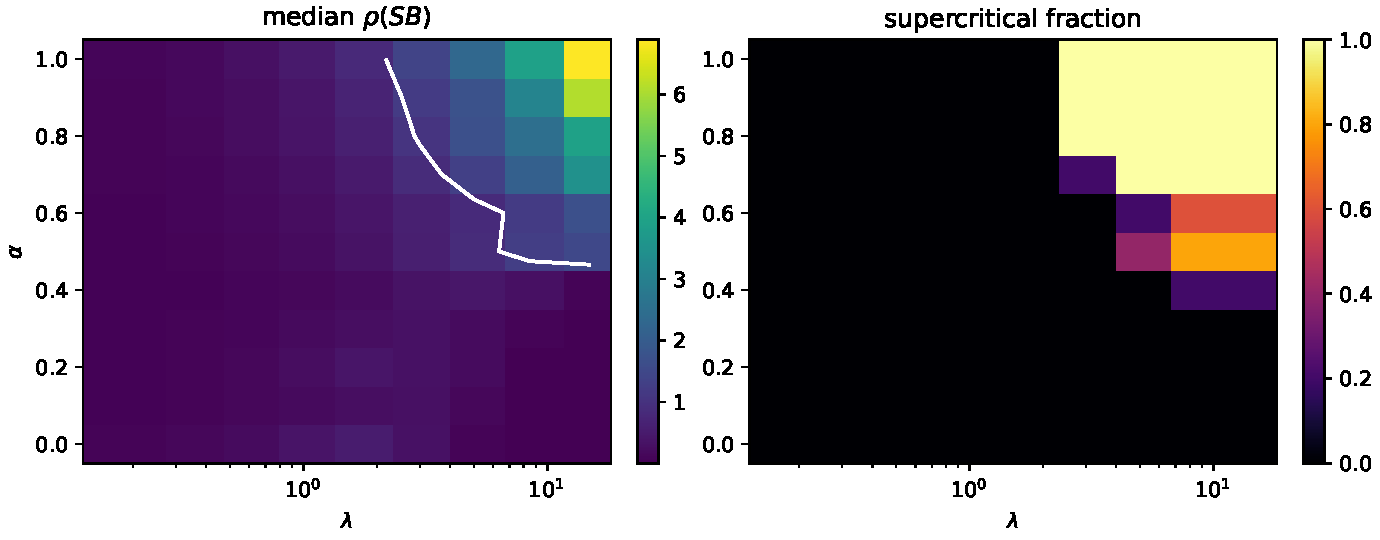
\includegraphics[width=\linewidth]{figures/phase_wedge.pdf}
\caption{The $\alpha\times\lambda$ plane. Left: median $\rho(SB)$ with the
$\rho=1$ contour in white --- non-monotone along the bottom edge (criticality
escape), unbounded along the top. Right: fraction of games per cell with
$\rho \ge 1$ --- the supercritical wedge, frontier descending in $\alpha$.
Artifact: \texttt{phase\_map\_surface.json}.}
\label{fig:wedge}
\end{figure}

Two consistency checks the map passes: the escape mechanism predicts no Hopf
bifurcation of logit dynamics in full potential games ($B = B^\top$ makes the
$SB$ spectrum real; verified exactly across the $\lambda$ grid), consistent
with cycles requiring non-potential structure \citep{hommes2012}; and the
$\alpha = 0$ row of every dissipation meter reads zero to machine precision at
all $\lambda$, as it must.

Both questions this section left open in v0.1 are now closed (unit
\texttt{science.frontier}). The peak location is a \emph{pure} scale fold:
$\sigma(\lambda, s\cdot u) = \sigma(s\lambda, u)$ is an algebraic identity
(checked numerically to error $0.0$), so $\rho$ depends on $\lambda$ and the
payoff scale only through their product and the peak is physical only in the
normalised coordinate. And $\lambda_c(\alpha)$ --- defined as the
verified-unique crossing of the fixed-family median-$\rho$ curve, with
single-crossing checked at every level before bisection --- is a clean
monotone-descending frontier: $7.8$ at $\alpha = 0.55$ down to $3.0$ at
$\alpha = 0.80$, with no median crossing below $\alpha \approx 0.5$ by
$\lambda = 15$ at 40-game sampling (the earlier 5-game map's onset at
$\alpha = 0.5$ is sampling variability of the median, recorded as such).
